\chapter{Testovanie algoritmu pri zmene počtu tried}\label{chap:implementation}

V predošlých kapitolách sme si ukázali ako sa mení presnosť a rýchlosť tréningu pri zmene počtu trénovacích obrázkov pre 6 novel tried a taktiež sa nám podarilo poslednú fázu tréningu(fine tuning) 8 násobne zrýchliť. Teraz využijeme náš zrýchlený algoritmus a pozrieme sa na to ako sa mení presnosť a rýchlosť pri zvyšovaní počtu počtu novel tried.

\section{Fine-tuning na base + novel triedach}

Najprv vyskúšame ako sa nám mení presnosť pri zvyšovaní počtu novel tried, pri ponechaní detekcie 15 base tried, rovnako ako doteraz. Neskôr si vyskúšame spraviť fine-tuning len na novel triedach, čo by malo zvýšiť našu presnosť pre novel triedy, s tým, že base triedy nebudeme detegovať. 

Pre jednoduchšie a rýchlejšie pridávanie nových tried som napísal zopár scriptov. Popíšem postup ako pridať novú triedu do datasetu: 

Anotované obrázky pre nové triedy stiahneme z roboflow~\cite{roboflow} vo formate Pascal VOC XML. Pre pridanie novej triedy do datasetu treba rozdeliť anotované obrázky na trénovacie a testovacie. Stačí keď presunieme všetky anotované obrázky do priečinka \texttt{datasets/VOC2007/ImageSets/Main/test}. Následne spustíme script \texttt{datasets/VOC2007/ImageSets/Main/divideDataset.py}, ktorý rozdelí anotované obrázky do priečinkov train a test. Keďže na fine-tuning nebudeme potrebovať príliš trénovacích obrázkov tak do priečinka train presunieme 30 obrázkov a zvyšok necháme v priečinku test. Potom treba spustiť script, datasets/VOC2007/ImageSets/Main/addNewClass.py, ktorý pridá nové obrázky do textových súborov trainval.txt a test.txt a presunie anotácie do \texttt{datasets/VOC2007/Annotations} a obrázky do \texttt{datasets/VOC2007/JPEGImages}.

Potom treba spustiť script \texttt{datasets/prepare\_voc\_few\_shot.py}, ktorý vytvorí textové súbory pre jednotlivé k-shot tréningy pre každú triedu. Vo formáte \texttt{box\_kshot\_názov\_triedy\_train.txt}, každý z týchto súborov obsahuje k názvov náhodných obrázkov z danej triedy, ktoré berie z textového suboru trainval.txt a následne sa trénuje a validuje počas fine-tuningu len na nich. Všetky obrázky v testovacej množine sú využité pri testovaní, na vyhodnotenie nášho modelu. 

Rozhodol som sa používať pri tomto testovaní 10-shot detekciu, pretože dosahuje  vysokú presnosť, rozptyl medzi presnoťou jednotlivých tried je nízky a vieme ju vykonať po našom zrýchlení pomerne rýchlo za cca hodinu. 

Nové triedy som vyberal úplne náhodne a keďže závisí presnosť detekcie na ich podobnosti s base triedami, ukážeme si taktiež AP50 pre jednotlivé novel triedy.

\subsubsection{10 novel tried}

Na obrázkoch \ref{fig:image6001} až \ref{fig:image6004} vidíme príklady anotovaných obrázkov pre novo pridané novel triedy.

\begin{figure}[H]
\centering
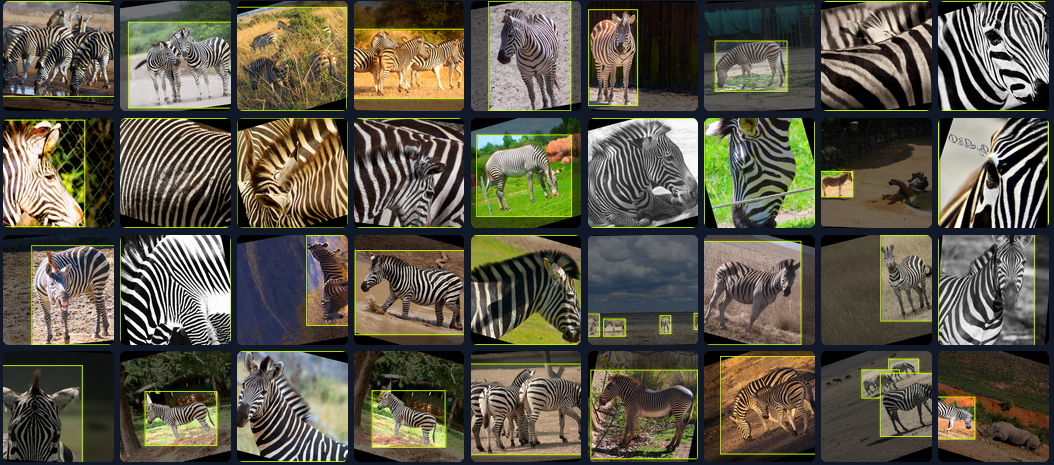
\includegraphics[width=\textwidth]{images/zebra_example_annotations.png}
\caption{Príklady anotovaných obrázkov pre triedu zebra}
\label{fig:image6001}
\end{figure}

\begin{figure}[H]
\centering
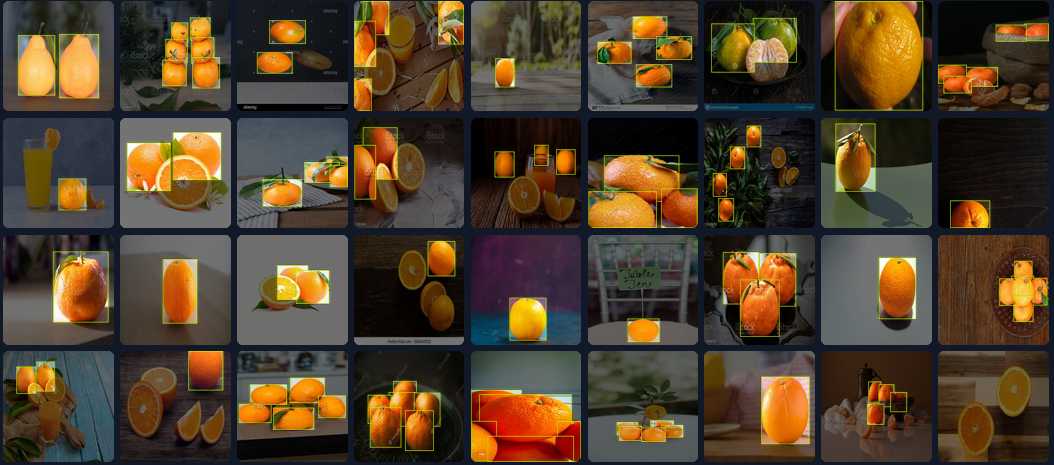
\includegraphics[width=\textwidth]{images/orange_example_annotations.png}
\caption{Príklady anotovaných obrázkov pre triedu pomaranč}
\label{fig:image6002}
\end{figure}

\begin{figure}[H]
\centering
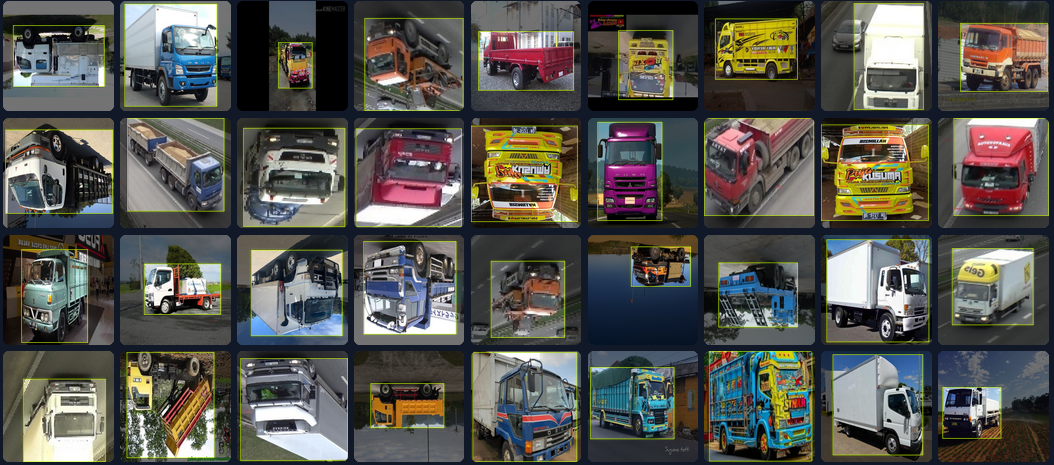
\includegraphics[width=\textwidth]{images/truck_example_annotations.png}
\caption{Príklady anotovaných obrázkov pre triedu nákladné vozdilo}
\label{fig:image6003}
\end{figure}

\begin{figure}[H]
\centering
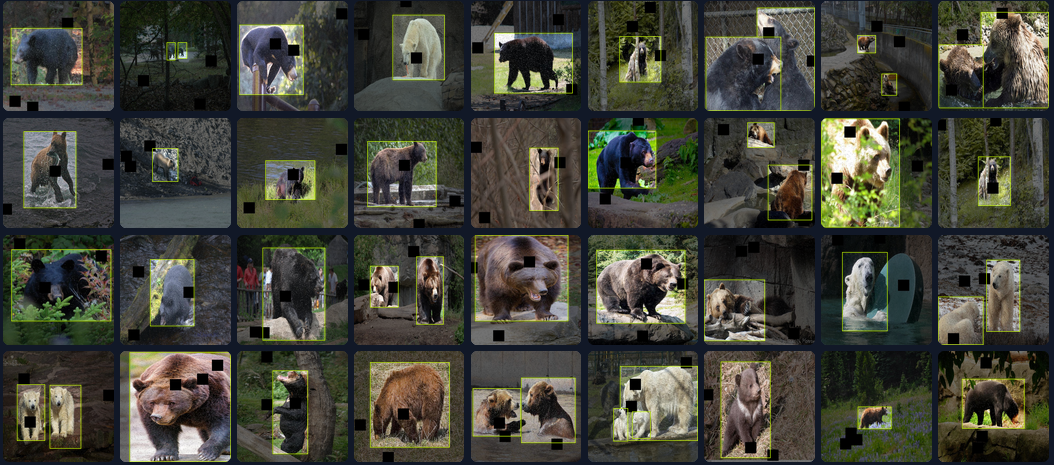
\includegraphics[width=\textwidth]{images/bear_example_annotations.png}
\caption{Príklady anotovaných obrázkov pre triedu medveď}
\label{fig:image6004}
\end{figure}

Tréning trval 1 hodinu, 7 minút a 51 sekúnd. Dĺžka tréningu sa nám o trochu zvýšila oproti 6 novel triedam a taktiež nám trochu klesla presnosť. Ako vidíme na obrázku \ref{fig:image611} presnosti sú pomerne dobre rozložené a nové triedy si držia solidnú presnosť. 

\begin{figure}[H]
\centering
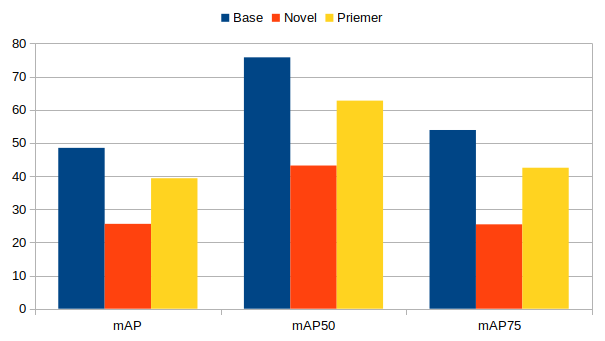
\includegraphics[width=\textwidth]{images/10novel_chart.png}
\caption{Graf presností na testovacích dátach pre 10 novel tried + 15 base tried pri 10-shot detekcii.}
\label{fig:image61}
\end{figure}

\begin{figure}[H]
\centering
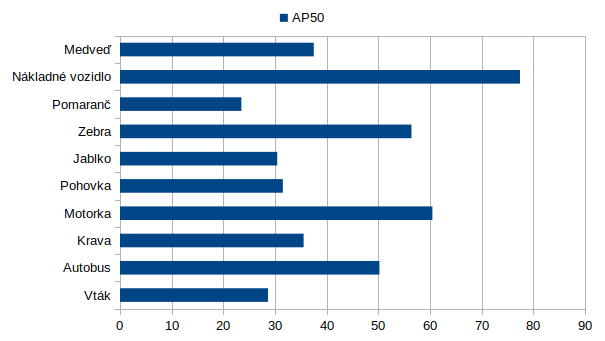
\includegraphics[width=\textwidth]{images/10novel_classes_chart.png}
\caption{AP50 na testovacích dátach pre 10 novel tried pri 10-shot detekcii}
\label{fig:image611}
\end{figure}

\begin{table}[H]
\begin{tabular}{|l|c|c|c|}
\hline
\textbf{Presnosť} & \textbf{Base} & \textbf{Novel} & \textbf{Priemer} \\
\hline
mAP & 48.508 & 25.594 & 39.342 \\
mAP50 & 75.803 & 43.18 & 62.754 \\
mAP75 & 53.901 & 25.442 & 42.517 \\
\hline
\end{tabular}
\centering
\caption{Tabuľka presností na testovacích dátach pre 10 novel tried + 15 base tried pri 10-shot detekcii.}
\label{tab:table60}
\end{table}

\subsubsection{15 novel tried}

Na obrázkoch \ref{fig:image6005} - \ref{fig:image6009} vidíme príklady anotovaných obrázkov pre novo pridané novel triedy.

\begin{figure}[H]
\centering
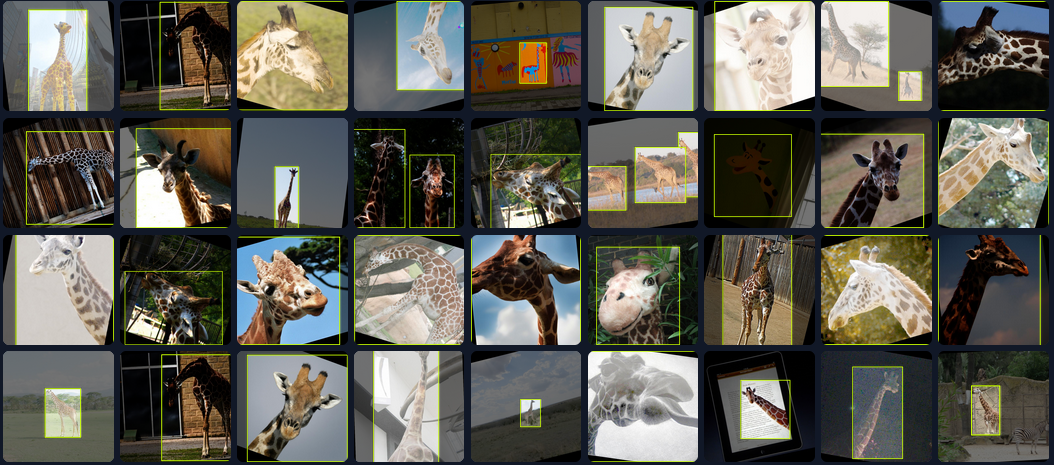
\includegraphics[width=\textwidth]{images/giraffe_example_annotations.png}
\caption{Príklady anotovaných obrázkov pre triedu žirafa}
\label{fig:image6005}
\end{figure}

\begin{figure}[H]
\centering
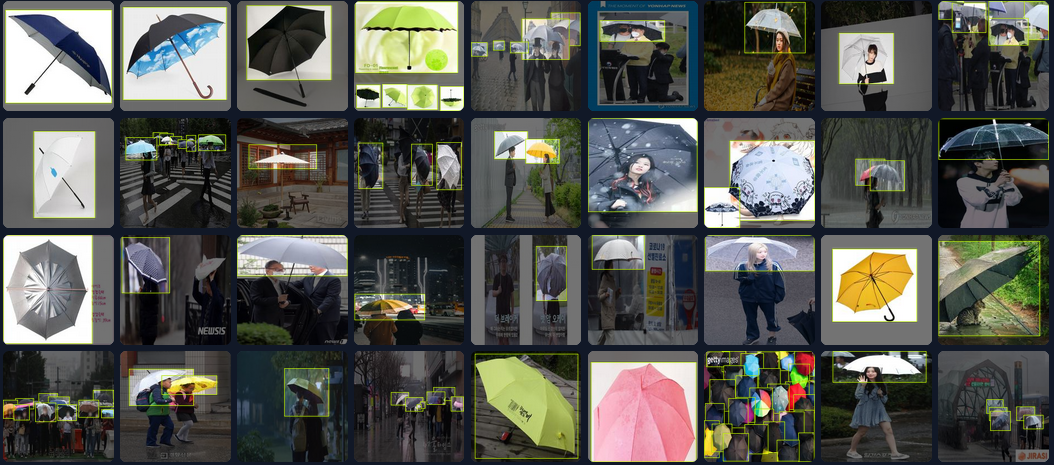
\includegraphics[width=\textwidth]{images/umbrella_example_annotations.png}
\caption{Príklady anotovaných obrázkov pre triedu dážnik}
\label{fig:image6006}
\end{figure}

\begin{figure}[H]
\centering
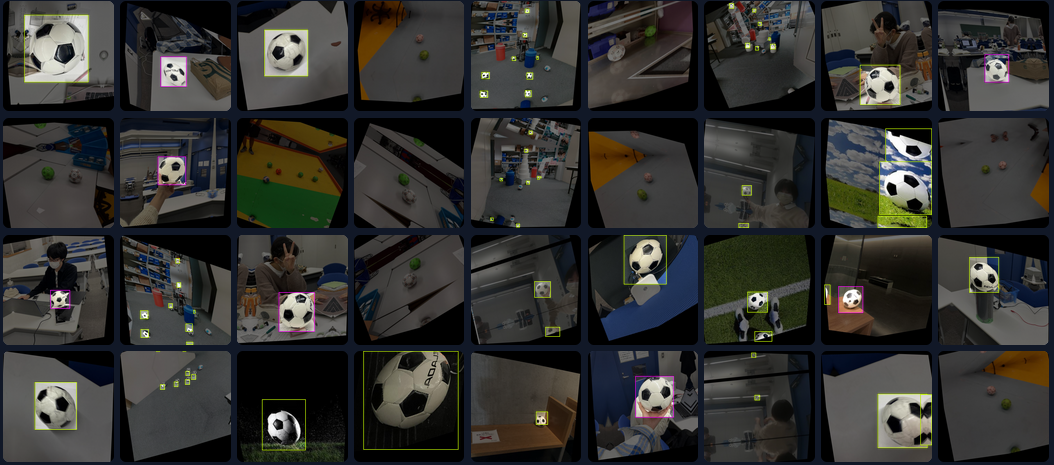
\includegraphics[width=\textwidth]{images/football_example_annotations.png}
\caption{Príklady anotovaných obrázkov pre triedu futbalová lopta}
\label{fig:image6007}
\end{figure}

\begin{figure}[H]
\centering
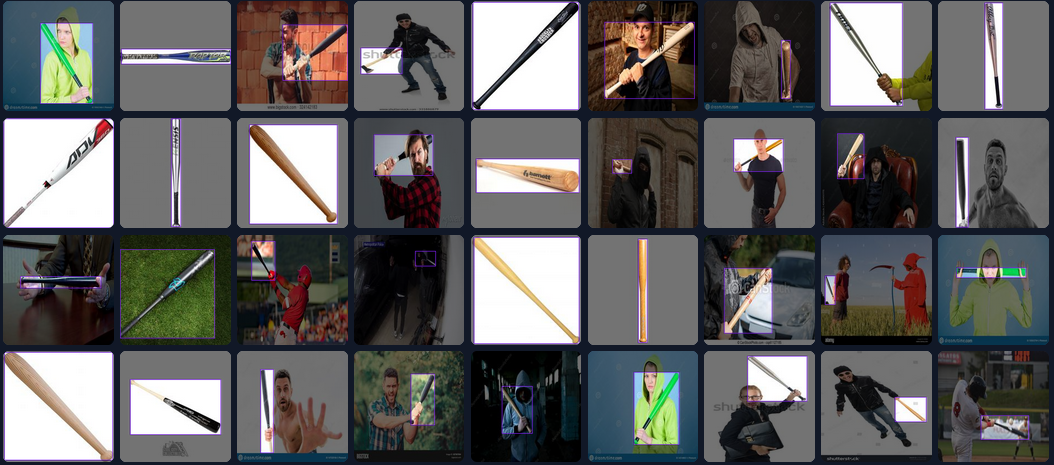
\includegraphics[width=\textwidth]{images/bat_example_annotations.png}
\caption{Príklady anotovaných obrázkov pre triedu basebalová pálka}
\label{fig:image6008}
\end{figure}

\begin{figure}[H]
\centering
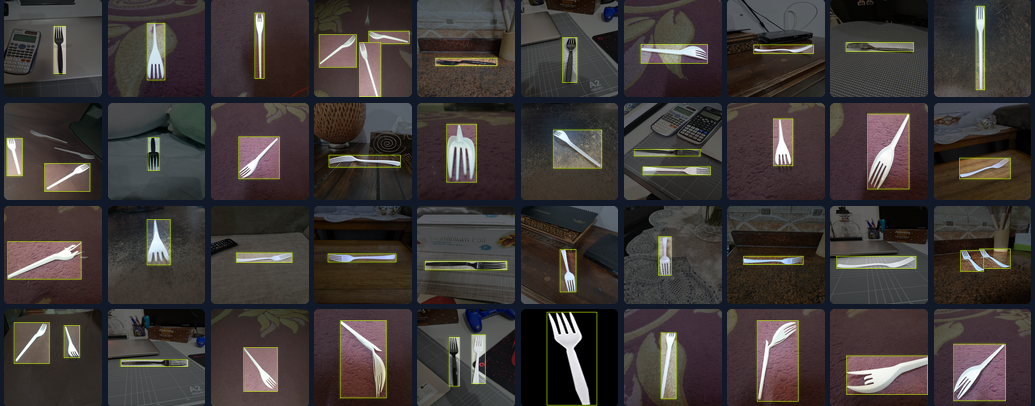
\includegraphics[width=\textwidth]{images/fork_example_annotations.png}
\caption{Príklady anotovaných obrázkov pre triedu vydlička}
\label{fig:image6009}
\end{figure}

Tréning trval 1 hodinu, 18 minút a 41 sekúnd. V tabuľke \ref{tab:table61} a na obrázku \ref{fig:image63} vidíme presnosť pri 15 novel triedach. Vidíme, že presnosť nám klesla a na obrázku \ref{fig:image612} vidíme, že sa nám taktiež zvýšila odchílka v presnosti medzi triadami a niektoré triedy majú dosť nízku presnosť, trieda dážnik má takmer nulovú.

\begin{figure}[H]
\centering
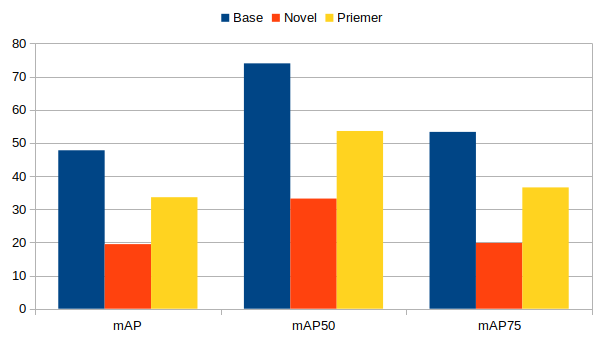
\includegraphics[width=\textwidth]{images/15novel_chart.png}
\caption{Graf presností na testovacích dátach pre 15 novel tried + 15 base tried pri 10-shot detekcii.}
\label{fig:image63}
\end{figure}

\begin{figure}[H]
\centering
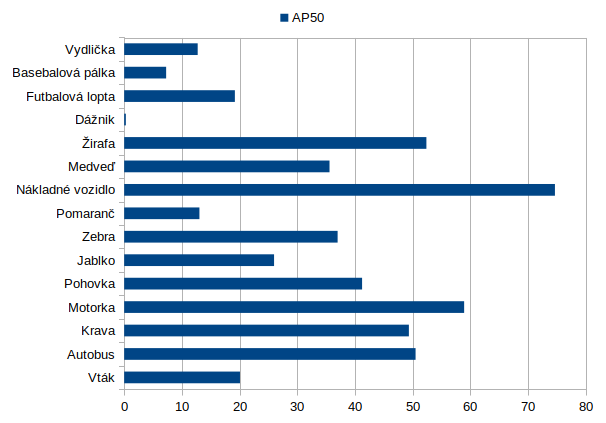
\includegraphics[width=\textwidth]{images/15novel_classes_chart.png}
\caption{AP50 na testovacích dátach pre 15 novel tried pri 10-shot detekcii.}
\label{fig:image612}
\end{figure}

\begin{table}[H]
\begin{tabular}{|l|c|c|c|}
\hline
\textbf{Presnosť} & \textbf{Base} & \textbf{Novel} & \textbf{Priemer} \\
\hline
mAP & 47.779 & 19.471 & 33.625 \\
mAP50 & 73.987 & 33.208 & 53.597 \\
mAP75 & 53.33 & 19.824 & 36.577 \\
\hline
\end{tabular}
\centering
\caption{Tabuľka presností na testovacích dátach pre 15 novel tried + 15 base tried pri 10-shot detekcii.}
\label{tab:table61}
\end{table}

\subsubsection{20 novel tried}

Na obrázkoch \ref{fig:image6010} - \ref{fig:image6014} vidíme príklady anotovaných obrázkov pre novo pridané novel triedy.

\begin{figure}[H]
\centering
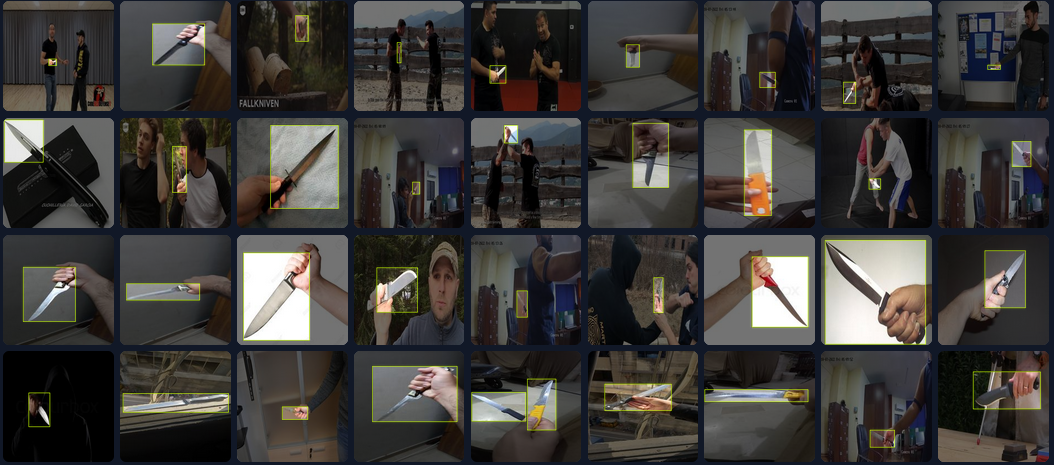
\includegraphics[width=\textwidth]{images/knife_example_annotations.png}
\caption{Príklady anotovaných obrázkov pre triedu nôž}
\label{fig:image6010}
\end{figure}

\begin{figure}[H]
\centering
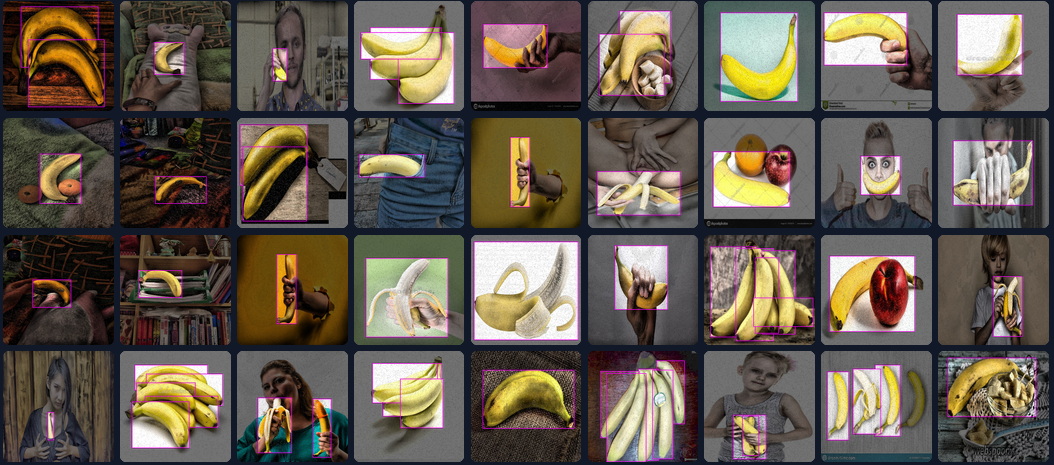
\includegraphics[width=\textwidth]{images/banana_example_annotations.png}
\caption{Príklady anotovaných obrázkov pre triedu banán}
\label{fig:image6011}
\end{figure}

\begin{figure}[H]
\centering
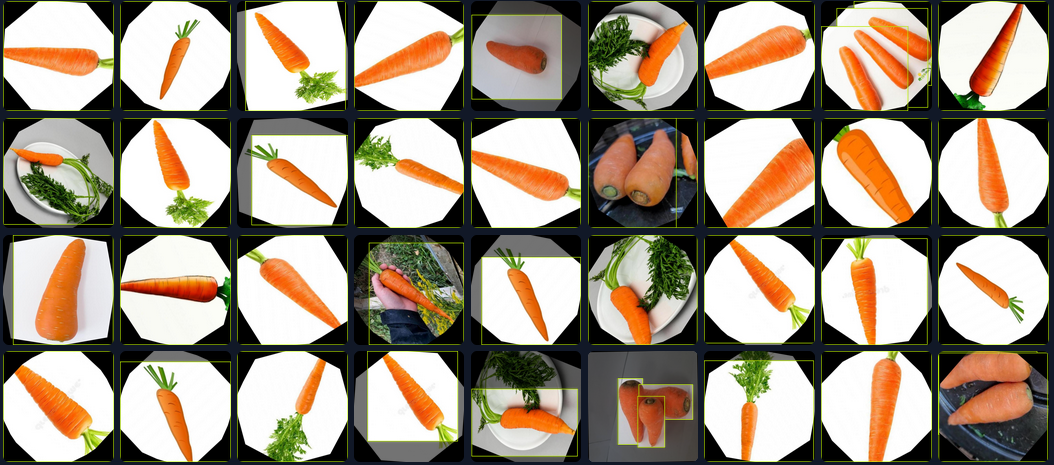
\includegraphics[width=\textwidth]{images/carrot_example_annotations.png}
\caption{Príklady anotovaných obrázkov pre triedu mrkva}
\label{fig:image6012}
\end{figure}

\begin{figure}[H]
\centering
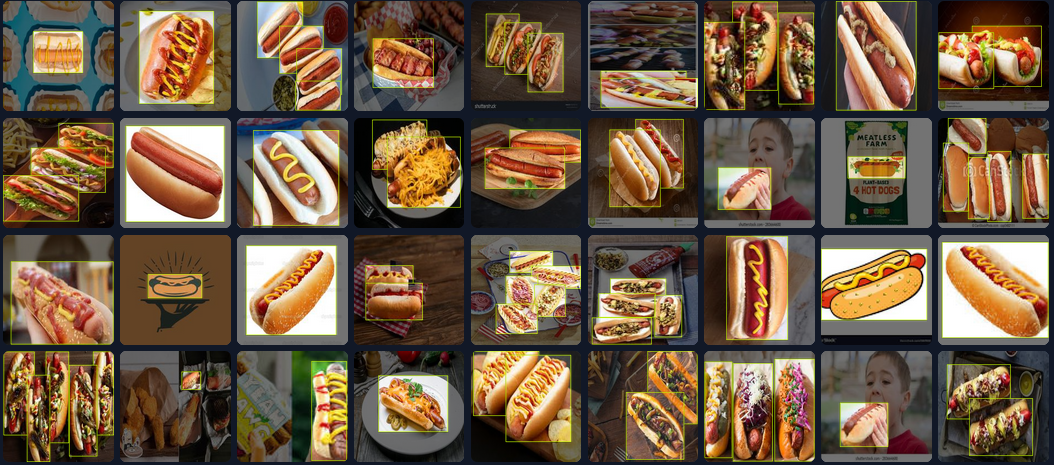
\includegraphics[width=\textwidth]{images/hotdog_example_annotations.png}
\caption{Príklady anotovaných obrázkov pre triedu hotdog}
\label{fig:image6013}
\end{figure}

\begin{figure}[H]
\centering
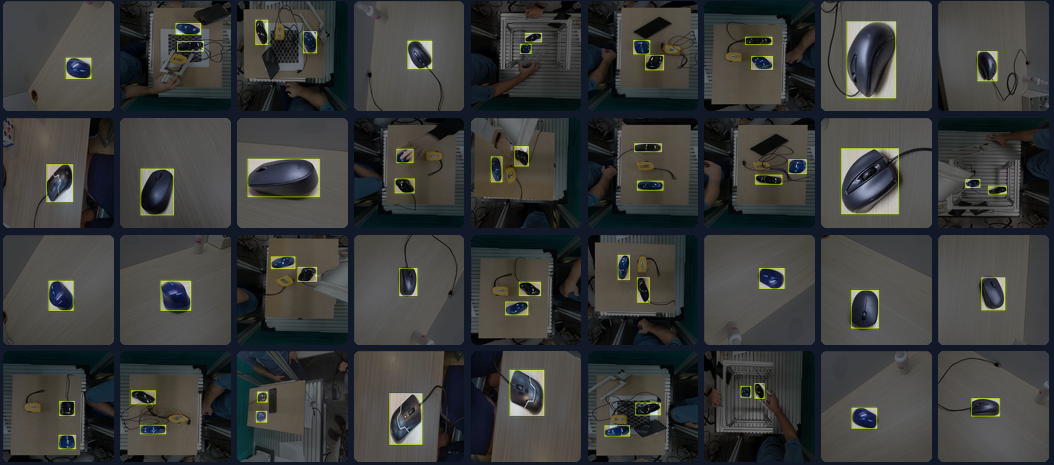
\includegraphics[width=\textwidth]{images/computer_mouse_example_annotations.png}
\caption{Príklady anotovaných obrázkov pre triedu počítačová myš}
\label{fig:image6014}
\end{figure}

Tréning trval 1 hodinu, 19 minút a 23 sekúnd. V tabuľke \ref{tab:table62} a na obrázku \ref{fig:image65} vidíme presnosť pri 20 novel triedach. Na obrázku \ref{fig:image613} vidíme presnosť jednotlivých novel tried. Nové triedy Hotdog, Nôž, Dážnik a Basebalová pálka majú veľmi nízku presnosť AP50 pod 10.

\begin{figure}[H]
\centering
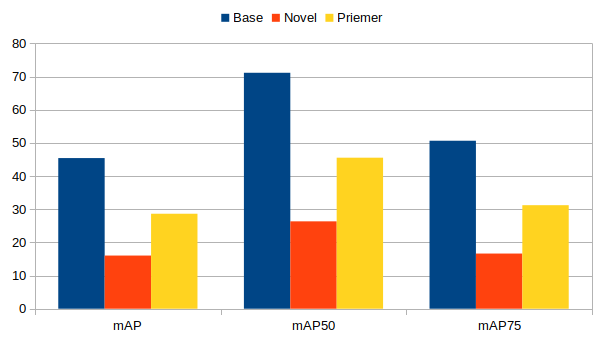
\includegraphics[width=\textwidth]{images/20novel_chart.png}
\caption{Graf presností na testovacích dátach pre 20 novel tried + 15 base tried pri 10-shot detekcii.}
\label{fig:image65}
\end{figure}

\begin{figure}[H]
\centering
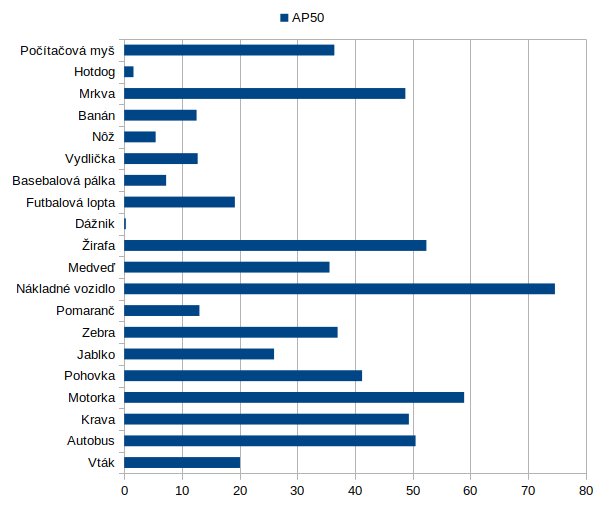
\includegraphics[width=\textwidth]{images/20novel_classes_chart.png}
\caption{AP50 na testovacích dátach pre 20 novel tried pri 10-shot detekcii.}
\label{fig:image613}
\end{figure}

\begin{table}[H]
\begin{tabular}{|l|c|c|c|}
\hline
\textbf{Presnosť} & \textbf{Base} & \textbf{Novel} & \textbf{Priemer} \\
\hline
mAP & 45.432 & 16.031 & 28.631 \\
mAP50 & 71.154 & 26.336 & 45.544 \\
mAP75 & 50.659 & 16.635 & 31.217 \\
\hline
\end{tabular}
\centering
\caption{Tabuľka presností na testovacích dátach pre 20 novel tried + 15 base tried pri 10-shot detekcii.}
\label{tab:table62}
\end{table}

Vidíme, že pri zvyšovaní počtu tried nám presnosť nášho tréningu stále klesá. Vyskúšame zvýšiť počet iterácií tréningu, keďže počet trénovacích obrázkov sa nám zvýšil, skúsime zvýšiť počet iterácií pri 20 novel triedach na dvojnásobok, teda aj čas tréningu bude dvojnásobne dlhý a porovnáme ich presnosť. 

\begin{figure}[H]
\centering
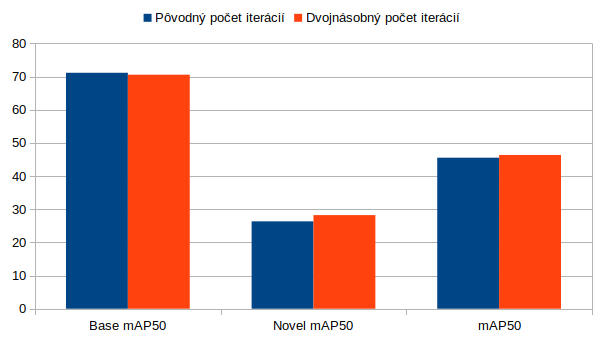
\includegraphics[width=\textwidth]{images/compare_20novel.png}
\caption{Porovnanie presnoti na testovacích dátach 10-shot detekcie s 20 novel triedami + 15 base triedami s pôvodným a dvojnásobným počtom iterácii}
\label{fig:image66}
\end{figure}

Ako vidíme na obrázku \ref{fig:image66}, pri zdvojnásobení počtu iterácií sa nám presnosť trochu zvýšila avšak len minimálne na úkor zdvojnásobenia dĺžky tréningu, takže to nebolo príliš efektívne.  

\subsubsection{Vyhodnotenie}

\begin{figure}[H]
\centering
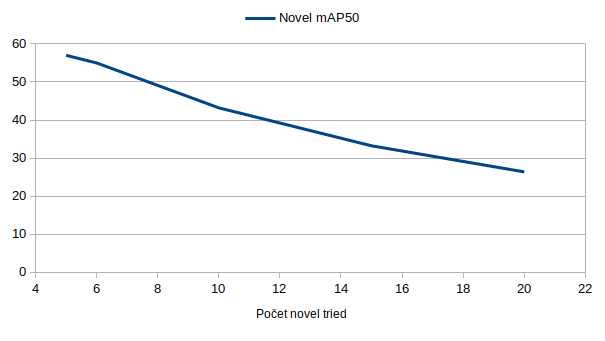
\includegraphics[width=\textwidth]{images/more_novel_results.png}
\caption{Presnosť 10-shot detekcie na testovacích dátach vzhľadom k počtu novel tried}
\label{fig:image67}
\end{figure}

Ako vidíme na obrázku \ref{fig:image67} presnosť nám pri zvyšovaní počtu novel tried konštantne klesá. Ak by sme chceli udržať našu presnosť pri viacej novel triedach ideálne by bolo natrénovať viacej modelov každý pre detekciu iných tried. 

\section{Fine-tuning len na novel triedach}

Ak nepotrebujeme detegovať base triedy, môžu byť využité len pri 1.fáze tréningu (base tréning), na predtrénovanie celej siete. Následný fine-tuning môžme robiť len na novel triedach, čo by malo zvýšiť presnosť ich detekcie.

Vyskúšame spraviť 10-shot fine-tuning na 20 novel triedach, bez base tried a porovnáme presnosť detekcie pri detekcii 20 novel tried spolu s 15 base triedami. 

\begin{figure}[H]
\centering
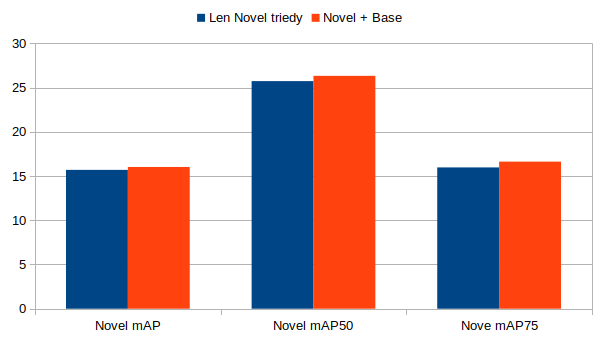
\includegraphics[width=\textwidth]{images/only_novel_compare_chart.png}
\caption{Graf porovnania presnosti na testovacích dátach pre fine-tuning bez a s base triedami pri 10-shot detekcii}
\label{fig:image69}
\end{figure}

\begin{table}[H]
\begin{tabular}{|l|c|c|}
\hline
\textbf{Presnosť} & \textbf{Len Novel triedy} & \textbf{Novel + Base} \\
\hline
Novel mAP & 15.696 & 16.031 \\
Novel mAP50 & 25.74 & 26.336 \\
Novel mAP75 & 15.978 & 16.635 \\
\hline
\end{tabular}
\centering
\caption{Tabuľka porovnania presnosti na testovacích dátach pre fine-tuning bez a s base triedami pri 10-shot detekcii}
\label{tab:table63}
\end{table}

Ako vidíme v tabuľke \ref{tab:table63} a na obrázku \ref{fig:image69} fine-tuning čisto na novel triedach nenaplnil naše očakávania a presnosť detekcie novel tried sa dokonca trochu znížila. 
